\subsubsection{\ac{pu} approximation}\label{subsec:pu_approximation}

\citet{chuang_debiased_2020} assume a \ac{pu} learning scenario, 
where positive samples and an unlabeled image dataset $p(x)$ are available.
Since positive samples may not be available in reality, 
the positive distribution $p^+$ is mimicked by data augmentations.

\citeauthor{chuang_debiased_2020}'s goal is to sample \acp{tn}.
They denote sampling bias the phenomenon of sampling \acp{fn} as illustrated in \autoref{fig:sampling_bias}a.
When randomly sampling negative samples from the data distribution $p(x)$ 
a negative sample can inherently belong to the same latent class as the anchor.
The negative effect of sampling bias on the model's performance is illustrated in \autoref{fig:sampling_bias}b.
Consequently, they propose a debiased contrastive objective that corrects for sampling \acp{fn} 
%i.e., the selection of negative samples that have the same label as the anchor, 
in an unsupervised scenario.
The idea is to generate positive samples using augmentations,
to sample negative samples $x^-$ from the data distribution $p(x)$
and to add a correction term for \acp{fn} in the loss function.

\begin{figure}%
    \centering
    \subfloat[\centering Visualization of sampling bias similar to \citet{chuang_debiased_2020}. Sampling $x_i^-$ from $p$ can result in \ac{fn}.]
    {{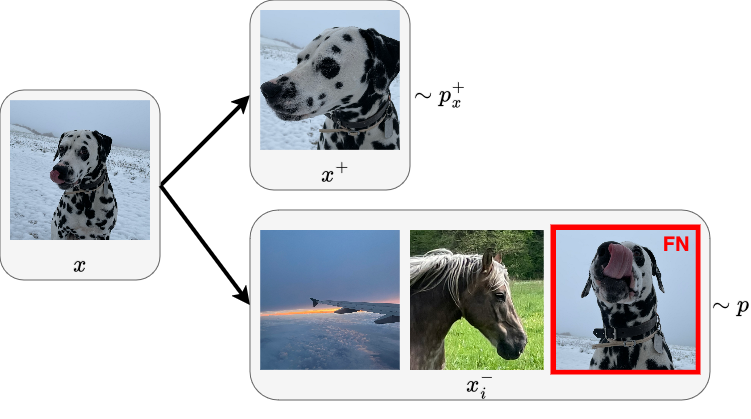
\includegraphics[width=5cm]{images/sampling_bias.png} }}%
    \qquad
    \subfloat[\centering Negative influence of sampling bias on accuracy from \citet{chuang_debiased_2020}.]{{\includegraphics[width=5cm]{images/debiased_sampling_accuracy.png} }}%
    \caption{Visualization of sampling bias and its effect on the model's performance.}%
    \label{fig:sampling_bias}%
\end{figure}